% !TeX program = pdfLaTeX
\documentclass[12pt]{article}
\usepackage{amsmath}
\usepackage{amsthm}
\usepackage{amssymb}
\usepackage{bbm}
\usepackage{graphicx,psfrag,epsf}
\usepackage{enumerate}
%\usepackage[numbers]{natbib}
\usepackage[nomarkers]{endfloat}
\usepackage{natbib}
\setcitestyle{numbers} 
\makeatletter % Reference list option change
\renewcommand\@biblabel[1]{#1. } % from [1] to 1
\makeatother %

\usepackage{booktabs}
\usepackage{longtable}
\usepackage{array}
\usepackage{adjustbox}
\usepackage{multirow}
\usepackage{subfig}
\usepackage[table,xcdraw]{xcolor}
\usepackage{wrapfig}
\usepackage{float}
%\usepackage{colortbl}
\usepackage[colorlinks]{hyperref}
\hypersetup{
  colorlinks=true,
  citecolor=black,
  linkcolor=black,
  urlcolor=blue}
  
\usepackage{pdflscape}
\usepackage{tabu}
\usepackage{threeparttable}
\usepackage{url} % not crucial - just used below for the URL

\usepackage{etoolbox}% http://ctan.org/pkg/etoolbox
\makeatletter
\patchcmd{\subsection}{\bfseries}{\relax}{}{}% Non-bold \subsection
\patchcmd{\subsubsection}{\bfseries}{\relax}{}{}% Non-bold \subsection
\makeatother


%\pdfminorversion=4
% NOTE: To produce blinded version, replace "0" with "1" below.
\newcommand{\blind}{0}

% DON'T change margins - should be 1 inch all around.
\addtolength{\oddsidemargin}{-.5in}%
\addtolength{\evensidemargin}{-.5in}%
\addtolength{\textwidth}{1in}%
\addtolength{\textheight}{1.3in}%
\addtolength{\topmargin}{-.8in}%

\newenvironment{definition}[1]% environment name 
{% begin code 
  \par\vspace{.75\baselineskip}\noindent 
  \textbf{Definition (#1)}\begin{itshape}% 
  \par\vspace{.5\baselineskip}\noindent\ignorespaces 
}% 
{% end code 
  \end{itshape}\ignorespacesafterend 
}

\providecommand{\tightlist}{%
  \setlength{\itemsep}{0pt}\setlength{\parskip}{0pt}}

\begin{document}

\def\spacingset#1{\renewcommand{\baselinestretch}%
{#1}\small\normalsize} \spacingset{1}



%%%%%%%%%%%%%%%%%%%%%%%%%%%%%%%%%%%%%%%%%%%%%%%%%%%%%%%%%%%%%%%%%%%%%%%%%%%%%%

\if0\blind
{
  \title{\bf Statistical Approaches to Automated Groove Engraved Area Identification
in 3D Bullet Land Scans}

  \author{
        Kiegan Rice \thanks{The authors gratefully acknowledge \ldots{}} \\
    Department of Statistics, Iowa State University\\
     and \\     Nathaniel Garton \\
    Department of Statistics, Iowa State University\\
     and \\     Ulrike Genschel \\
    Department of Statistics and CSAFE, Iowa State University\\
     and \\     Heike Hofmann \\
    Department of Statistics and CSAFE, Iowa State University\\
      }
  \maketitle
} \fi

\if1\blind
{
  \bigskip
  \bigskip
  \bigskip
  \begin{center}
    {\LARGE\bf Statistical Approaches to Automated Groove Engraved Area Identification
in 3D Bullet Land Scans}
  \end{center}
  \medskip
} \fi

\bigskip
\begin{abstract}

\end{abstract}

\noindent%
{\it Keywords:} 3 to 6 keywords, that do not appear in the title
\vfill

\newpage
\spacingset{1.45} % DON'T change the spacing!

\newcommand{\hh}[1]{{\color{orange}{#1}}}
\newcommand{\kr}[1]{{\color{teal}{#1}}}
\newcommand{\ug}[1]{{\color{purple}{#1}}}
\newcommand{\nate}[1]{{\color{olive}{#1}}}




\section{Background}

In forensic firearms analysis, visual feature comparison is used to
analyze bullets to address the same source-difference source problem.
Striation marks act as features which provide evidence to help determine
whether two bullets were propelled through the same gun barrel. Land
engraved areas (LEAs), alternating sections of the bullet that make the
closest contact with the gun barrel, are the primary source of striation
marks.

A cornerstone of forensic firearms analysis is that two bullets fired
through the same barrel will bear more similar striation marks on their
LEAs than two bullets fired from different barrels. The guideline used
to reach a same source determination, the AFTE Theory of Identification,
suggests that if two sets of striae are sufficiently similar ``the
likelihood another tool could have made the mark is so remote as to be
considered a practical impossibility" \citep{AFTE}.

The recent application of high resolution 3D scanning technology to
bullet LEAs coupled with concerns about the objectivity of visual
comparison have motivated the development of several image-analysis
algorithms which aim to complete automated, quantitative analyses of
bullet evidence
\citep[see][]{DeKinder1, DeKinder2, Bachrach1, Ma1, Chu1, Chu2, Hare1}.
The data used in such algorithms are high resolution 3D scans of LEAs,
such as that pictured in \autoref{LEA-scan}.

\begin{figure}
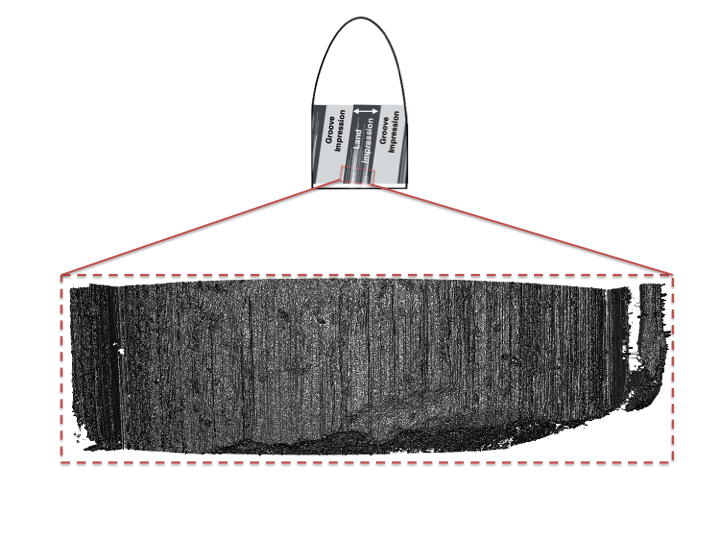
\includegraphics[width=\textwidth]{../images/3d_plot_top_context_breakoff.png}
\caption{An example of a high-resolution LEA scan captured on a Confocal Light Microscope.}
\label{LEA-scan}
\end{figure}

One such method, proposed by \citet{Hare1}, is a random forest algorithm
based on features calculated from 2D horizontal slices of the 3D images.
These slices, called profiles, have a data structure which is dominated
by the global structure of the bullet land: they are curved. The random
forest algorithm relies on processed versions of profiles which remove
the global curvature. This remaining pattern of peaks and valleys -
called a signature - is a much more useful representation of the
striations. The process of translating a 3D scan into a 2D signature is
demonstrated in \autoref{processing-process}.

\begin{figure}
\begin{minipage}[b]{0.45\linewidth}
    \raggedleft
    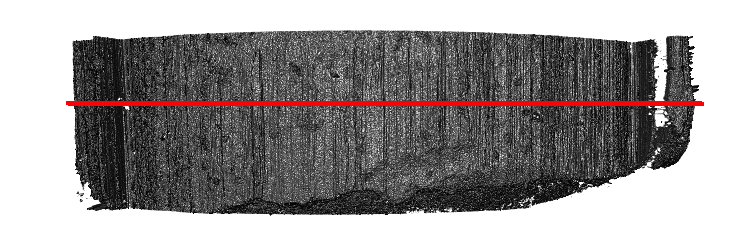
\includegraphics[width=\textwidth]{../images/3d_plot_top_crosscut.png}
    \centering
    Step 0: High-resolution 3D scan
\end{minipage}
\hspace{.2cm}
\begin{minipage}[b]{0.45\linewidth}
    \raggedright
    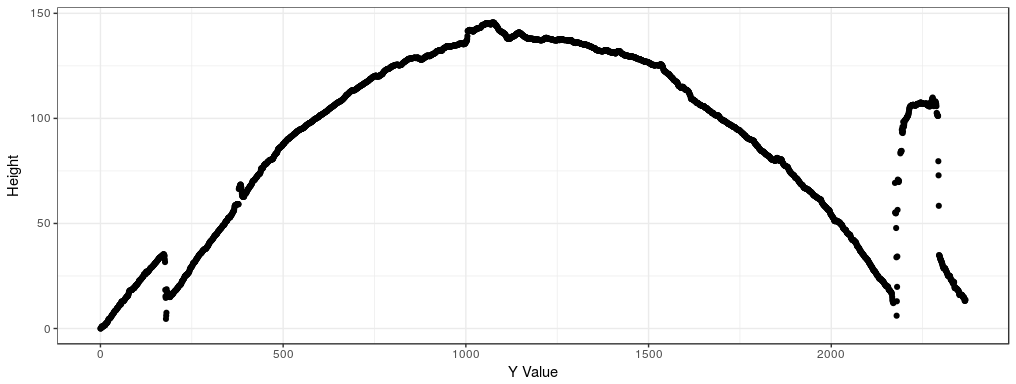
\includegraphics[width=\textwidth]{../images/Profile_1.png}
    \centering
    Step 1: Horizontal crosscut (profile)
\end{minipage}
\vspace{.6cm}

\begin{minipage}[b]{0.45\linewidth}
    \raggedleft
    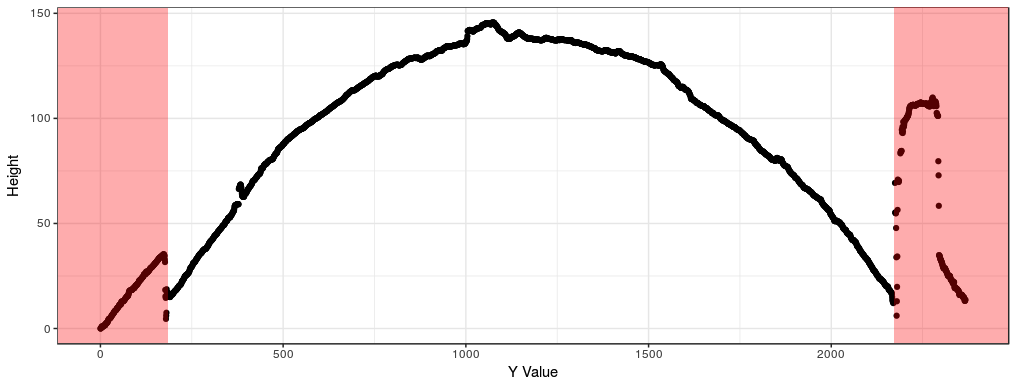
\includegraphics[width=\textwidth]{../images/Profile_1_red_grooves.png}
    \centering
    Step 2: GEA data removal
\end{minipage}
\hspace{.2cm}
\begin{minipage}[b]{0.45\linewidth}
    \raggedright
    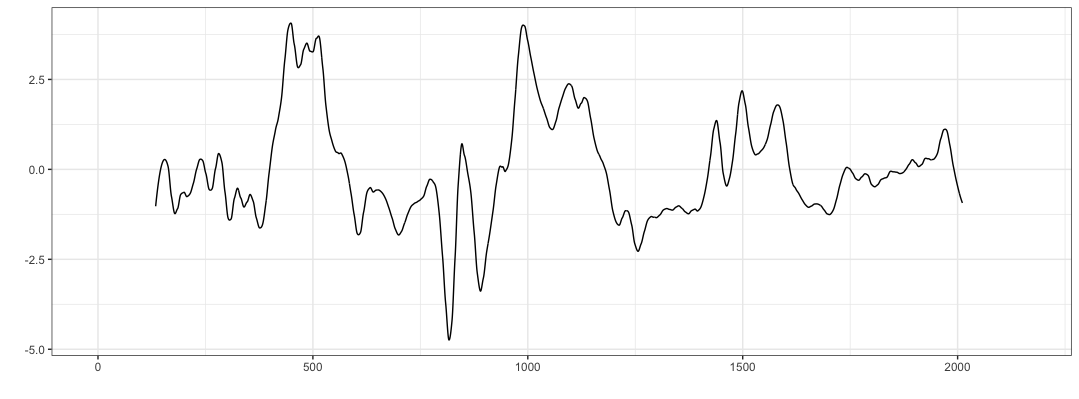
\includegraphics[width=\textwidth]{../images/signature.png}
    \centering
    Step 3: Extracted signature
\end{minipage}
\caption{The process of extracting a 2D signature from a high-resolution 3D scan of a land engraved area (LEA) on a bullet. Extraction of a signature is dependent on both the choice of horizontal crosscut and accuracy of GEA data removal procedure.}  
\label{processing-process}
\end{figure}

While removal of a curve from data is typically a straightforward
statistical problem, 3D scans of LEAs contain a unique data structure
which obfuscates this task. Currently accepted best practice for
collection of 3D images of bullet LEAs dictates that scanning begin and
end slightly past the edges of the LEA, in the neighboring groove
engraved areas (GEAs). GEAs are a secondary structure that need to be
removed before LEA signatures can be reliably extracted from data.

Correctly separating LEA and GEA data is one of the most challenging and
important aspects of data pre-processing. Without removing GEA data,
algorithms will be using extraneous data which can misrepresent the
character of the striations present on a given LEA. This type of
misrepresentation is demonstrated in \autoref{groove-no-groove}. In
order to distinguish between LEA and GEA data, we aim to identify
``shoulder locations'', the locations at which the LEA ends and the GEAs
begin.

\begin{figure}
\centering
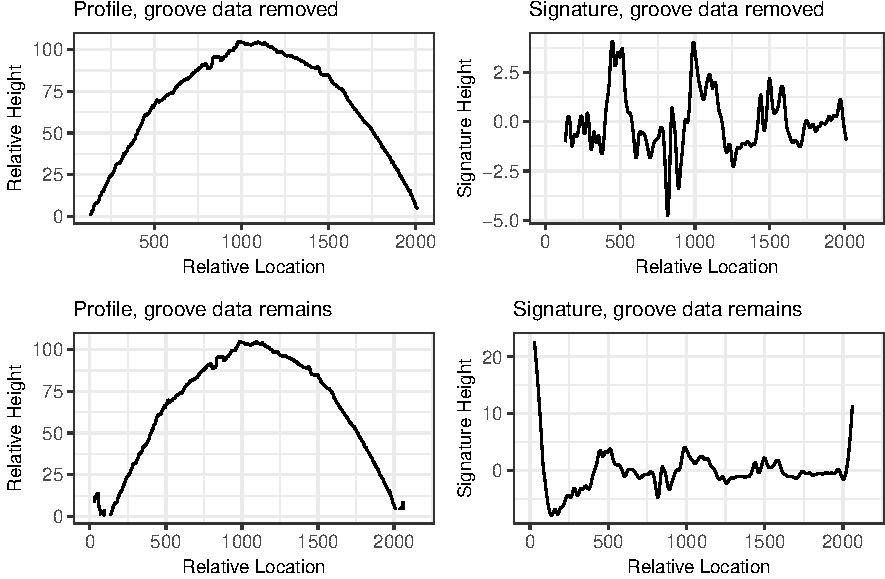
\includegraphics{writeup_files/figure-latex/groove-no-groove-1.pdf}
\caption{\label{groove-no-groove}An example of the impact failure to
remove GEA data can have on an extracted 2D signature. Important data
features are obfuscated in the signature by remaining GEA structure.}
\end{figure}

The method for shoulder location identification described in
\citet{Hare1}, based on data smoothing and local minima, fails to
reliably separate the GEA data from LEA data. The following work first
describes an improved methodology based on robust statistical methods
for fitting the global curvature of 2D profiles. Once global structure
is removed, two proposed approaches to identify shouler locations are
presented. Performance of both proposed shoulder location identification
methods are then compared with current approaches.

\section{Data Source}

The data used consist of high resolution 3D scans of bullet LEAs from
three separate test sets: Hamby Set 44 \citep{Hamby}, Phoenix PD set,
and Houston-test set.

Hamby set 44 consists of 35 bullets fired from 10 consecutively rifled
Ruger P85 barrels. There are two known bullets for each of the ten
barrels, as well as 15 additional questioned bullets. Each fired bullet
in Hamby Set 44 has 6 LEAs; every LEA was scanned for each of the 35
bullets, producing data for 210 individual land engraved areas. Two
lands -- Barrel 9, Bullet 2, Land 3 and Unknowns, Bullet L, Land 5 --
were removed from consideration due to ``tank rash''. Tank rash results
from a bullet striking the bottom of a water recovery tank after exiting
the barrel, thereby creating marks on the land that are not due to the
contact with the barrel.

The Phoenix PD set consists of 33 bullets fired from 8 barrels
\kr{more information on the type of barrels?}. There are three known
bullets for each of the eight barrels, as well as 9 additional
questioned bullets. There are 6 LEAs for each of the fired bullets,
producing a total of 198 individual land engraved areas.

The Houston-test set consists of 45 bullets fired from at least 10
barrels \kr{more information on the type of barrels?}. There are three
known bullets for each of the ten barrels, as well as 24 questioned
bullets that are fired from a combination of the 10 known barrels and
additional, out-of-set barrels. There are 6 LEAs for each of the fired
bullets, producing a total of 414 individual land engraved areas.

The 3D scans of each test set were captured with a Sensofar Confocal
light microscope at 20x magnification resulting in a resolution of 0.645
microns per pixel. These LEAs were scanned at Iowa State University's
High Resolution Microscopy Facility, and the scans are stored in 3D
format as x3p files, conforming to the ISO5436-2 standard
\citep{ISO5436}. A visualization of the data gathered for a single LEA
is seen in \autoref{LEA-scan}. Physically, each land is approximately 2
millimeters in width; as such, data structures for a single LEA can
contain more than 3 million individual data points.

A crosscut was extracted from each scan by identifying an optimal
crosscut using \texttt{x3p\_crosscut\_optimize} in the
\texttt{bulletxtrctr} package in \texttt{R} \cite{bulletxtrctr}. Then,
an averaged profile was calculated by averaging across ten consecutive
crosscuts which fall directly to either side of the optimal crosscut
identified. Shoulder location methods are applied to these averaged
profile, for a total of 820 profiles across the three test sets.

\section{Methodology}

\subsection{Global Structure Removal}

The first stage of our GEA removal process focuses on removing the
bullet curvature from each profile. GEAs on the edge of each LEA
represent a change in the data structure typically characterized by a
sharp increase in measured height values (see
\autoref{groove-no-groove}). Accurate removal of the primary structure
should accentuate these characteristics, which can then be used to
separate the LEA from the GEAs.

Although bullets are circular, the pressure they are subjected to in the
process of being fired out of a gun can often result in LEAs that are
not perfectly circular. In addition, the angle at which the LEAs are
scanned by operators can mean profiles are tilted or misshapen. Directly
modeling the data as if the bullet is circular may then be unreasonable
to remove the structure accurately across a whole profile. Thus, more
flexible non-parametric locally weighted regression (LOESS) is a natural
choice for removing the structure.

The flexibility of LOESS methods, while attractive here, often results
in an unduly large effect of GEA data on the estimated structure. To
mitigate this problem we employ a robust LOESS \citep{Cleveland1}.
Robust LOESS fits models by iteratively downweighting high residual
values to reduce the influence of outliers which deviate the most from
the main data structure. In the context of LEA profiles, robust LOESS
will iteratively downweight data points with high residuals, typically
those from the GEA which deviate most severely from the overall bullet
curvature.

Traditional robust LOESS can be implemented using the
\texttt{locfit.robust} function in the \texttt{locfit} package in
\texttt{R} \cite{locfit}. An example of the difference in both predicted
values and residual structure between \texttt{loess} and
\texttt{locfit.robust} can be seen in \autoref{loess-vs-locfit}.

\begin{figure}
\centering
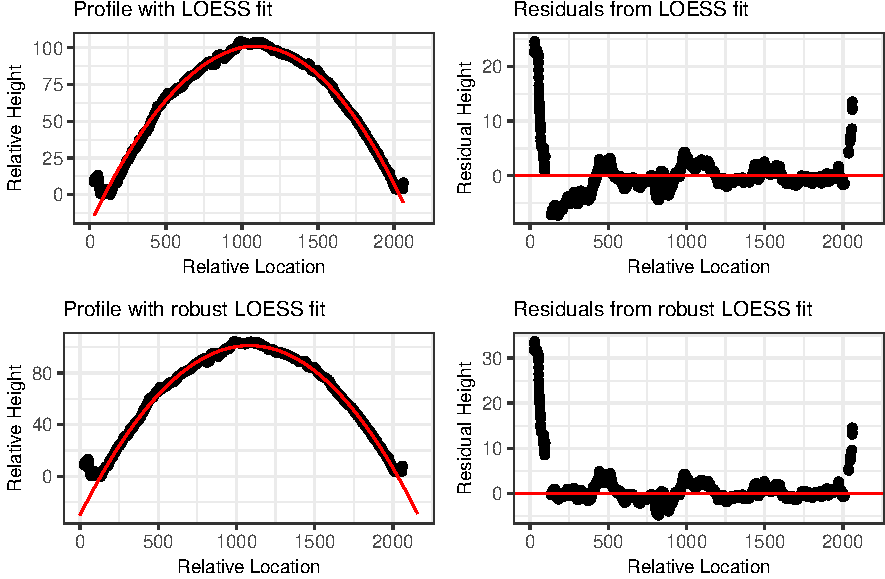
\includegraphics{writeup_files/figure-latex/loess-vs-locfit-1.pdf}
\caption{\label{loess-vs-locfit}An example of the difference between
traditional LOESS fit and robust LOESS fit to an LEA profile from Hamby
set 44. While the GEA structure present is relatively minor, even the
small improvement in model fit with robust LOESS results in
significantly different residual structures.}
\end{figure}

When applied to LEAs from Hamby set 44, the traditional robust LOESS
procedure appears to work well. However, the method fails to mitigate
effects when striations are deeper or GEA structures are more
pronounced, such as those in the Houston-test set, seen in
\autoref{houston-locfit}.

\begin{figure}
\centering
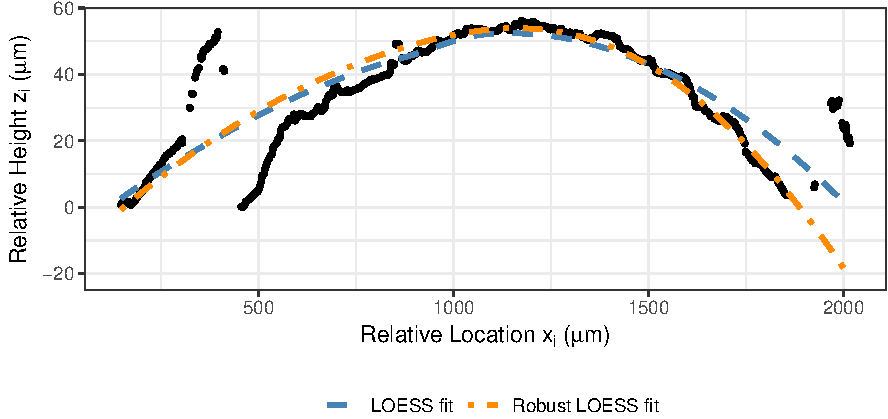
\includegraphics{writeup_files/figure-latex/houston-locfit-1.pdf}
\caption{\label{houston-locfit}An example of the difference between
traditional LOESS fit and robust LOESS fit to an LEA profile from the
Houston-test set. While the smaller GEA structure on the right side is
accounted for using the robust procedure, the larger GEA structure on
the left is still problematic.}
\end{figure}

Thus, we instead apply an adapted version of the traditional robust
LOESS procedure which focuses on iteratively reducing the influence of
only positive residuals. The procedure is as follows:

\begin{enumerate}

\item Fit a LOESS model with $span = 1$ to an entire LEA profile to predict $height$ using values of $x$. Assign weights of $1$ to each data point for this fitting procedure.  
\item Obtain predicted values of $height$ from the model fit in step 1.  
\item Calculate residual values using the predicted $height$ values.  
\item Calculate bisquare weights for each residual value using the following formula:  
$$\max(1 - (residual/(6*MAR))^2, 0)^2,$$   where MAR is the median absolute residual for the profile.  
\item Assign weights to each data point according to its residual value. If the residual value is positive, assign the bisquare downweight. If the residual is zero or negative, leave the weight at 1.  
\item Repeat steps 1-5 with updated weights at each iteration for $k$ iterations, with 20 iterations as the default.  
\item After $k$ iterations of updating the weight vector, fit a LOESS model with $span = 1$ and obtained predicted and residual values for $height$.  

\end{enumerate}

This procedure is attractive in the LEA profile context because the main
influence of GEA data is to pull predictions up towards the higher GEA
height values. Downweighting high residuals for only those that fall
above the fitted line will iteratively bring the fitted line down
towards the LEA structure. While this is a small procedural difference,
the results are dramatic. The same LEA pictured in
\autoref{houston-locfit} can be seen again with updated predictions in
\autoref{houston-adapted-rlo}.

\begin{figure}
\centering
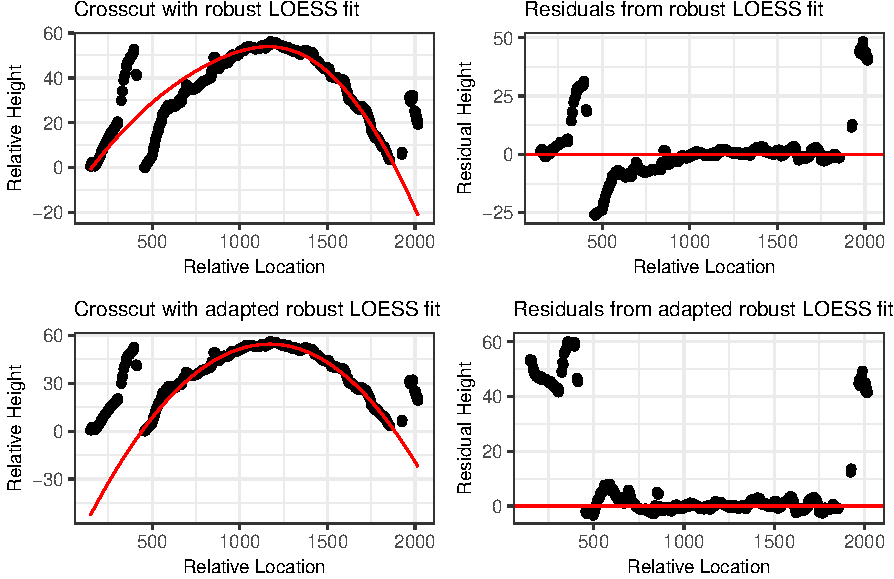
\includegraphics{writeup_files/figure-latex/houston-adapted-rlo-1.pdf}
\caption{\label{houston-adapted-rlo}An example of the difference between
robust LOESS fit and adapted robust LOESS fit to an LEA profile from the
Houston-test set. Iteratively downweighting only positive residuals
results in a significantly different fit which accounts for GEA
structures on both the left and right.}
\end{figure}

The utility of this adaptation can be seen in
\autoref{adapted-rlo-shift}, which shows the mean shift in predicted
values from the robust LOESS to the adapted robust LOESS for our three
different test sets of interest. While the difference is almost
imperceptible for Hamby set 44, the Phoenix PD and Houston-test sets
demonstrate visible downward shifts near both the left and right
boundaries.

\begin{figure}
\centering
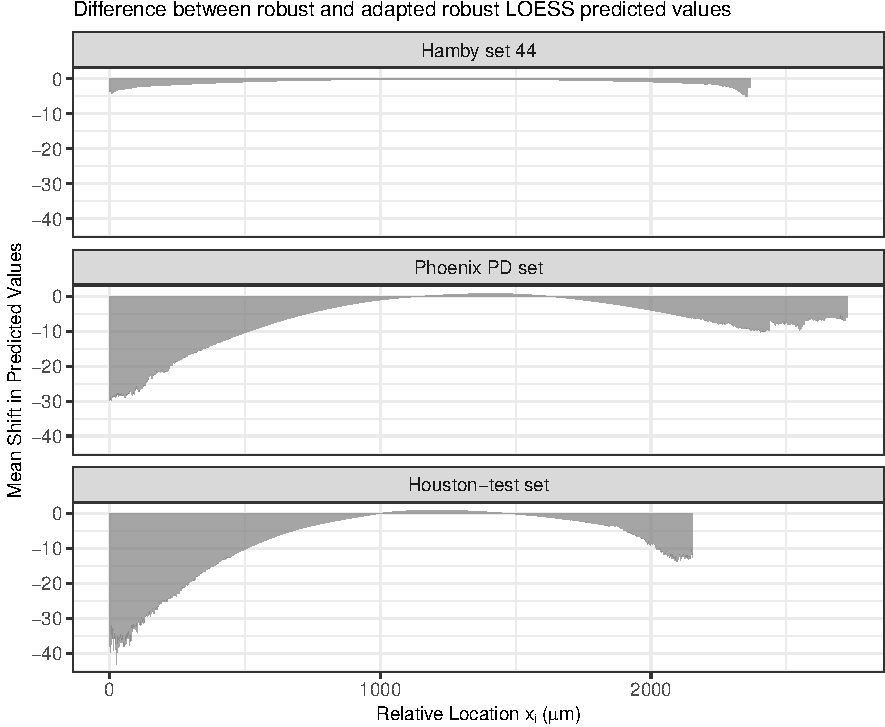
\includegraphics{writeup_files/figure-latex/adapted-rlo-shift-1.pdf}
\caption{\label{adapted-rlo-shift}Mean shift in predictions when
applying the adapted robust LOESS procedure in place of the traditional
robust LOESS procedure. For Hamby set 44, predictions are, on average,
very similar. The Phoenix PD and Houston-test sets have more significant
downwards shifts in predictions near the left and right boundaries.}
\end{figure}

Once the adapted robust LOESS procedure has been applied to remove the
bullet curvature of the LEA, the resulting residuals should have
relatively different distributions between LEA and GEA data. Points in
the LEA will fall more closely to the fitted line, while points in the
GEA will typically have high, positive residuals.

The subsequent prediction methods for shoulder location are based on the
residuals calculated from the adapted robust LOESS fit to the global
structure of each profile. One method, using supervised two-class
classification techniques, aims to classify each data point as being
part of the LEA or GEA. The second approach is an unsupervised method
based on changepoint analysis that seeks to identify data points where
the distribution of the residuals changes.

\subsection{Two-Class Classification}

Shoulder location can be predicted by first classifying data points as
one of two classes (``LEA'' or ``GEA''), and subsequently gathering the
range of values classified as ``LEA'' points.

Classification into ``LEA'' or ``GEA'' is first approached by a process
of feature engineering based on adapted robust LOESS residuals. While
the residuals themselves should have different height patterns,
residuals alone are not enough to classify data with high accuracy.

As already demonstrated by the differences in \autoref{loess-vs-locfit}
and \autoref{houston-locfit}, certain ammunition or barrel types may
result in more pronounced striae on an LEA. Thus, standardization of
features is imperative for transferability of fitted model parameters.
The LEA scan context requires some non-traditional standardization
practices.

For example, consider the distribution of residual values resulting from
adapted robust LOESS. There is reason to believe that the distribution
will be quite skewed, which means a standard deviation will not be a
good proxy for the spread of the distribution. Thus, rather than the
standard deviation, we consider instead the standard deviation of
residual values from the middle 50\% of \(x\) values present on the
scan. This alternative acts as a proxy for the depth of striae on each
LEA, with higher standard deviations found for lands with deeper striae.
Standardizing residual values by this proxy puts all residuals on a
similar scale.

For variables which instead deal with differences in the \(x\)
direction, such as depth from the center of a scan, values will be
mapped to a \((0, 1)\) range, with the maximum \(x\) location on the
scan acting as the divisor.

The full list of features developed are as follows:

\begin{itemize}

\item[] \texttt{rlo\_resid\_std}: Robust LOESS residual value, standardized by dividing by standard deviation of residual values from middle 50\% of \textbf{x} values.  

\item[] \texttt{(rlo\_resid\_std$\mathbf{)^2}$}: Squared term of \texttt{rlo\_resid\_std}.  

\item[] \texttt{side}: Whether data point is to left or right of median $x$ value.  

\item[] \texttt{depth\_std}: Distance of data point from median $x$ value, standardized by dividing by maximum $x$ value (a proxy for the range of $x$).  

\item[] \texttt{side:depth\_std}: Interaction between \texttt{side} and \texttt{depth\_std} variables.  

\item[] \texttt{xint1\_std}: Predicted x intercept of robust LOESS on left side of land, standardized by dividing by maximum $x$ value (a proxy for the range of $x$).  

\item[] \texttt{xint2\_std}: Predicted x intercept of robust LOESS on right side of land, standardized by dividing by maximum $x$ value (a proxy for the range of $x$).  

\item[] \texttt{range\_50\_std}: Range of residual values within a 50-point window around data point, standardized by dividing by standard deviation of residual values from middle 50\% of $x$ values.  

\item[] \texttt{numNA\_50}: Number of missing values within a 50-point window around data point.  

\item[] \texttt{ind\_2mad}: Indicator of whether \texttt{rlo\_resid} is greater than \texttt{2*MAD(rlo\_resid)}.  

\item[] \texttt{numpos\_50}: Number of positive residual values within a 50-point window around data point.  

\item[] \texttt{ind\_edges}: Indicator of whether data point is to the left of \texttt{xint1} or to the right of \texttt{xint2}. Values between \texttt{xint1} and \texttt{xint2} receive a value of 0, while values on the outside of the two values receive a value of 1.  

\end{itemize}

Examples of the distributions of some of these features can be seen in
\autoref{lasso-features}.

\begin{figure}
\centering
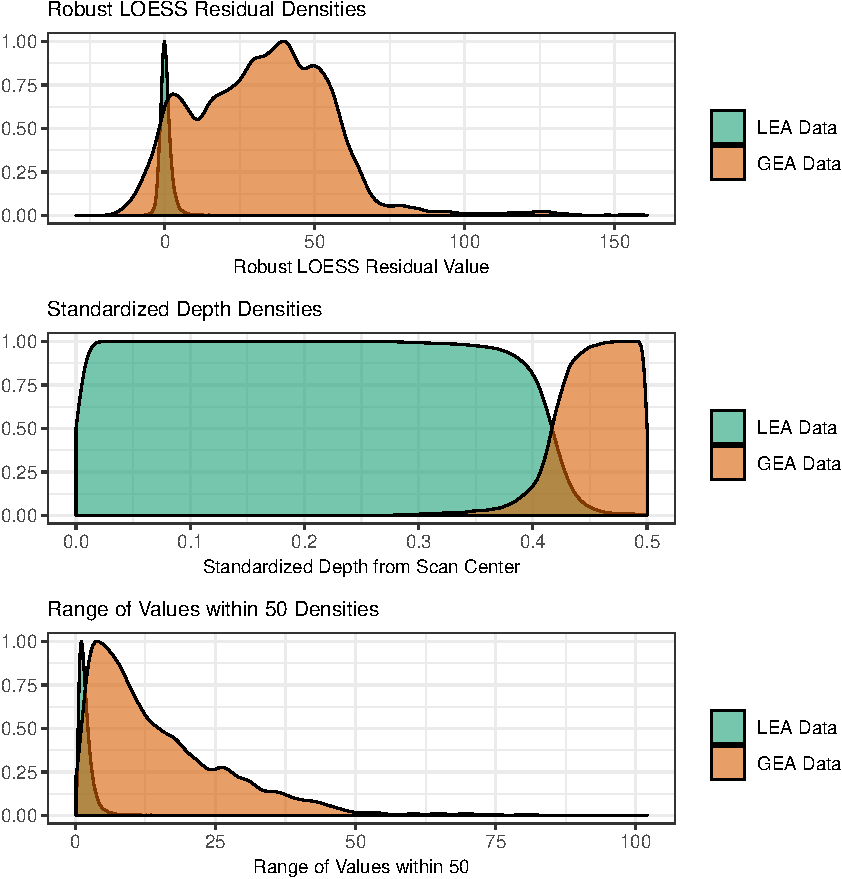
\includegraphics{writeup_files/figure-latex/lasso-features-1.pdf}
\caption{\label{lasso-features}Example distributions of features used in
two-class classification. While depth shows the most clear separation
between GEA and LEA data, it alone will not suffice to classify data
correctly. While other distributions are relatively tight for LEA, there
is still significant overlap with the wider GEA distributions.}
\end{figure}

The developed features can be used in the fit of a logistic LASSO model,
which is a form of penalized regression. LASSO parameter values for
\(p\) covariates are found by identifying:

\[
\hat{\beta}_{\lambda}^q = \stackrel{\arg\min}{\beta \in \mathbb{R}^p} \left\{  (Y - X\beta)'(Y - X\beta) + \lambda \sum_{j=1}^{p}|\beta_j|^q\right\}
\] which adds a penalty to the traditional ordinary least squares
minimization problem, and uses a tuning parameter \(\lambda\).

Cross-validated LASSO models were fit using the \texttt{cv.glmnet}
function in the \texttt{glmnet} package \cite{glmnet}. For each model,
parameter values from the model with \(\lambda_{1se}\) were used.
\(\lambda_{1se}\), a standard when using LASSO, is the tuning parameter
which results in the simplest model that still has cross-validation
error within one standard deviation of the best model.

Two separate models were fit: ``LASSO Basic'', which uses each of the
features listed above, and ``LASSO Full'', which uses each of the
features along with pairwise interactions for each of them. These
parameter values were trained on the Hamby set 44 data. The resulting
parameter values were used to calculate predicted values between 0 and
1; the closer to 1, the higher probability of membership in the ``GEA''
class.

Traditional two-class classification techniques call for finding an
\textbf{equal error rate cutoff} to classify the predicted values for
each data point into each of the two classes; i.e., values above a
certain cutoff are classified as part of the ``GEA'' class, and values
below the cutoff are classified as part of the ``LEA'' class. However,
since scans are primarily of the land engraved area, there is
significant class imbalance in our response categories. This unbalanced
response means that any criterion used to determine a reasonable cutoff
value for classification needs to be adjusted to account for differences
in the size of the response classes. The larger class size of ``LEA''
means an equal error rate would allow for more false negatives (i.e.,
more ``GEA'' data points being classified as ``LEA'') - exactly what we
are trying to avoid.

Thus, instead of looking for the cutoff that gives raw equal error rate
(where sensitivity and specificity are equal), we found an equal error
rate based on the overall number of data points. This allows for an
equal \textbf{number} of errors in each category, rather than equal
\textbf{percentage} of errors. This tactic more fairly penalizes points
that should be classified ``GEA'' but are predicted to be ``LEA''.

The final process for shoulder location identification is as follows:

\begin{enumerate}
\item Use \texttt{robust\_loess\_fit} to remove bullet curvature.
\item Calculate features based on $x$ locations and residual height values from \texttt{robust\_loess\_fit}. 
\item Use fit parameter values from either (a) lassobasic or (b) lassofull models to calculate probabilities of membership in GEA class.
\item Apply cutoff of (a) .33 or (b) .34 to classify higher probabilities as GEA data points, and lower probabilities as LEA data points.
\item Gather the $x$ range of points classified as LEA data points. These are the final shoulder location preditions.  
\end{enumerate}

This process results in two methods for shoulder location identification
in the \texttt{R} package \texttt{bulletxtrctr}: ``lassobasic'' and
``lassofull''.

\subsection{Bayesian Changepoint Analysis}

The idea behind the changepoint approach is that within either the left
GEA, right GEA, or the LEA, the global structure is consistent and can
either be described by a line with zero slope, a line with positive
slope for the right GEA, or a line with negative slope for the left GEA.
Finding the points where the GEAs and LEA meet is treated as a problem
of model selection. That is, the best fitting statistical model, in
terms of the magnitude of the likelihood, should be the one which
assumes that the points at which the global structure changes align with
where the GEAs and LEA meet. This approach was proposed in the more
general context of Bayesian changepoint detection in
\citet{stephens1994}. Thus, the points of global structural change are
what we will call changepoints. Thus, our model will be defined in a
piecewise fashion. In practice there are also complex additional
patterns which may exist for a number of reasons, but this large scale
structural assumption remains generally reasonable. The complex smaller
scale patterns can be thought of as the dependence in the data after
accounting for the global structure. Because of the nature of the model
which we consider, it becomes necessary for computational reasons to
perform a couple of additional data preprocessing steps. Specifically,
we will scale the residuals from the robust LOESS procedure, and we will
impute missing values. In the next section, we describe the model that
we will use to identify changepoints, after which we will describe the
estimation procedure which we use. Details of the additional data
preprocessing steps can be found in the appendix.

\subsubsection{Bayesian Model Formulation}

Before introducing the model, we introduce some notation. First, let
\(\{Y(x_i): i = 1,2, ..., n\}\) denote the set of random variables
representing the residuals from the robust LOESS procedure at the values
\(x_i\). For simplicity, also assume that \(x_1 < x_2 < ... < x_n\).
Also, let \(c_l\) be the value of the left changepoint and \(c_r\) be
the value of the right changepoint. Here, the left changepoint is where
the left GEA meets the LEA, and the right changepoint is where the right
GEA meets the LEA. Also, denote the median centered \(x\) values as
\(x'_i = x_i - \tilde{x}\) where \(\tilde{x}\) is the median \(x\)
value. As mentioned in the previous paragraph, the complex small scale
patterns, such as the striae, will be modeled through a covariance
structure on the data that will be allowed to differ between each GEA
and between the GEAs and LEA. We will construct the covariance matrices
from the exponential covariance function
\(K(x, x';\sigma, \ell) = \sigma^2 e^{-\frac{|x - x'|}{\ell}} = cov(Y(x), Y(x'))\).
The differences in covariance matrices for the GEAs and LEA will be
reflected in the parameters \(\sigma\) and \(\ell\). The data model that
we consider is then,

\begin{align}
(Y(x_1), Y(x_2), ..., Y(x_{k_1}))^{\top} &\sim N(\beta_{01}\mathbbm{1} + \beta_{11} x_{1:k_1}, \Sigma_1(\sigma_1, \ell_1)) \\
(Y(x_{k_1 + 1}), Y(x_{k_1 + 2}), ..., Y(x_{k_2}))^{\top} &\sim N(0, \Sigma_2(\sigma_2, \ell_2)) \\ 
(Y(x_{k_2 + 1}), Y(x_{k_2 + 2}), ..., Y(x_n))^{\top} &\sim N(\beta_{02}\mathbbm{1} + \beta_{12} x_{k_2 + 1:n}, \Sigma_3(\sigma_3, \ell_3)),
\end{align}

\noindent where \(x_{k_1} < c_l \leq x_{k_1 + 1}\) and
\(x_{k_2} < c_r \leq x_{k_2 + 1}\) Here, \(x_{1:k}\) denotes the column
vector \((x_1, x_2, ..., x_k)^\top\), and \(\mathbbm{1}\) denotes the
vector of ones. Indpendence is assumed between each of these three
distributions for simplicity. The parameters that need to be estimated
include the four mean parameters in the GEAs, the six covariance
parameters (two for each of the three areas), and the two changepoint
parameters, \(c_l\) and \(c_r\).

The above model encapsulates the essence of the approach. However, there
are a few difficulties. The first difficulty is that there are not
always two GEAs in a particular land. There may be one GEA, or the land
may only consist of the LEA. Thus, the above model is actually
conditional on there being two GEAs in the data. We also define models
for when there is one GEA on the left, one GEA on the right, or no GEAs.
The models are defined in an essentially identical way. Conditional on
there being only one GEA, the left GEA model is defined as,

\begin{align}
(Y(x_1), Y(x_2), ..., Y(x_{k}))^{\top} &\sim N(\beta_{0}\mathbbm{1} + \beta_{1} x_{1:k}, \Sigma_1(\sigma_1, \ell_1)) \\
(Y(x_{k + 1}), Y(x_{k + 2}), ..., Y(x_{n}))^{\top} &\sim N(0, \Sigma_2(\sigma_2, \ell_2)),
\end{align}

\noindent and the right GEA model is defined as,

\begin{align}
(Y(x_{1}), Y(x_{2}), ..., Y(x_{k}))^{\top} &\sim N(0, \Sigma_1(\sigma_1, \ell_1)) \\ 
(Y(x_{k + 1}), Y(x_{k + 2}), ..., Y(x_n))^{\top} &\sim N(\beta_{0}\mathbbm{1} + \beta_{1} x_{k + 1:n} \Sigma_2(\sigma_2, \ell_2)).
\end{align}

\noindent Finally, conditional on there being no GEAs in the data, the
model is simply

\begin{align}
(Y(x_{1}), Y(x_{2}), ..., Y(x_{n}))^{\top} &\sim N(0, \Sigma(\sigma, \ell)).
\end{align}

We see that estimating the changepoint locations also involves selecting
the most appropriate model. In order to avoid confusion, we have
slightly abused notation and, for example,
\(\Sigma_1(\sigma_1, \ell_1)\) as it is estimated in the two changepoint
model is \emph{not} the same as \(\Sigma_1(\sigma_1, \ell_1)\) from
either of the one changepoint models, and \(\Sigma_1(\sigma_1, \ell_1)\)
is also \emph{not} the same between the two one changepoint models. As
another example, \(\beta_0\) is \emph{not} the same between each of the
one changepoint models. So, to be clear, duplication of notation in
\emph{different} models is not meant to imply that those parameters are
shared between models.

Ultimately, these above four models are each individually fitted, and
each model above is given a prior. From there, we do model selection in
the formal Bayesian way, selecting number and location of changepoints
by maximizing the estimated posterior distribution.

In order to complete a Bayesian model specification, we need priors on
each of the parameters in each model as well as each model itself. We
will assume independence between each parameter a priori. For each
length scale \(\ell\), we will assume \(\ell \sim \text{Gamma}(3,5)\).
For each standard deviation, we will assume
\(\sigma \sim \text{Half-Normal}^{+}(0,1)\), where
\(\text{Half-Normal}^{+}(\cdot,\cdot)\) is notation for the normal
distribution restricted to the positive real numbers. For intercept
parameters, \(\beta_{01}, \beta_{02}, \beta_0 \sim N(0, 10)\). For the
slope parameters, the preceding trend deviates slightly. For any slope
that corresponds to the \emph{left} GEA, \(\beta_1\) or \(\beta_{01}\),
we will assume that the slope can not be positive. That is,
\(\beta_1, \beta_{01} \sim \text{Half-Normal}^{-}(0,10)\), where
\(\text{Half-Normal}^{-}(\cdot, \cdot)\) is notation for the normal
distribution restricted to the negative real numbers. Contrastingly, for
any slope that corresponds to the \emph{right} GEA, \(\beta_1\) or
\(\beta_{02}\), we will assume that the slope can not be negative. That
is, \(\beta_1, \beta_{01} \sim \text{Half-Normal}^{+}(0,10)\). For the
changepoint locations, we assume a uniform prior
\(\pi(c_l, c_r) \propto I(a < c_l < c_r - \gamma < b - \gamma)\). Here,
\(a\) and \(b\) are some values close to the edges of the data. How
close those values are to the edges is a parameter that is set manually.
Further, we include another hyperparameter, \(\gamma\), which can be set
so that the changepoints are not allowed to be too close to each other.
This is also a parameter that is set manually. Lastly, we assume a
uniform prior over all four models.

\subsubsection{Bayesian Model Estimation}

As was noted in \citet{stephens1994}, for any model including a
changepoint, the likelihood is not a smooth function of the changepoint
location. This is because, holding all other parameters fixed, shifting
the changepoint value will result in zero change to the likelihood until
it crosses the nearest point to the right or left, at which point the
likelihood makes a jump. This makes maximum likelihood estimation in the
standard way infeasible, but Bayesian estimation can be done in a fairly
straightforward way via Markov chain Monte Carlo (MCMC). The basic idea
is that, for each model, we can construct a two step Gibbs sampler. In
step 1 we sample from the posterior distribution of the mean and
covariance parameters given the changepoint locations, and in step 2 we
sample from the changepoint locations given the mean and covariance
parameters. Because of the non-conjugacy in our model, we perform both
sampling steps using a random walk Metropolis-Hastings (RWMH) step with
Gaussian proposals. For details on Gibbs sampling and the
Metropolis-Hastings algorithm see \citet{gelman2013}. It is also worth
mentioning that the zero changepoint model does not require Gibbs
sampling at all, and we perform estimation there using a RWMH algorithm.

We now provide the two basic steps of the Gibbs sampler for the two
changepoint case. The algorithms to sample from the other three models
are omitted, and are nearly identical except for the a smaller number of
parameters need to be sampled. Denote collection of mean and covariance
parameters for the left GEA as \(\theta_1\), the LEA as \(\theta_2\),
and the right GEA as \(\theta_3\). Then, at iteration \(t\) after warmup

\begin{enumerate}
\def\labelenumi{\arabic{enumi}.}
\tightlist
\item
  given changepoint locations \((c_l^{(t - 1)}, c_r^{(t - 1)})\), sample
  \((\theta_1^{(t)}, \theta_2^{(t)}, \theta_3^{(t)})\) using independent
  RWMH steps for each \(\theta_i\)
\item
  given \((\theta_1^{(t)}, \theta_2^{(t)}, \theta_3^{(t)})\), sample
  \((c_l^{(t)}, c_r^{(t)})\) using a single RWMH step.
\end{enumerate}

After running the MCMC for each model, parameter estimates and the most
likely model are jointly chosen according to the largest joint posterior
value. That is, we arrive at estimates
\((\hat{\theta}, \hat{M}) = \underset{(\theta, M)}{\operatorname{argmax}}{\log(p(\theta, M | Y))}\),
where \(M\) is the random variable associated with the choice of model,
\(\theta\) is the associated parameter vector for the appropriate model,
and \(Y\) is all of the available data. Additional MCMC details can be
found in the appendix.

The idea behind the changepoint approach is that within either the left
GEA, right GEA, or the LEA, the global structure is consistent and can
either be described by a line with zero slope, a line with positive
slope for the right GEA, or a line with negative slope for the left GEA.
Finding the points where the GEAs and LEA meet is treated as a problem
of model selection. That is, the best fitting statistical model, in
terms of the magnitude of the likelihood, should be the one which
assumes that the points at which the global structure changes align with
where the GEAs and LEA meet. This approach was proposed in the more
general context of Bayesian changepoint detection in
\citet{stephens1994}. Thus, the points of global structural change are
what we will call changepoints. Thus, our model will be defined in a
piecewise fashion. In practice there are also complex additional
patterns which may exist for a number of reasons, but this large scale
structural assumption remains generally reasonable. The complex smaller
scale patterns can be thought of as the dependence in the data after
accounting for the global structure. Because of the nature of the model
which we consider, it becomes necessary for computational reasons to
perform a couple of additional data preprocessing steps. Specifically,
we will scale the residuals from the robust LOESS procedure, and we will
impute missing values. In the next section, we describe the model that
we will use to identify changepoints, after which we will describe the
estimation procedure which we use. Details of the additional data
preprocessing steps can be found in the appendix.

\section{Results}

To assess the degree of improvement in automated shoulder location
identification, we want to quantify the impact each groove prediction
method has on the automated bullet matching algorithm's accuracy. Five
different shoulder location identification methods will be inserted into
the automated bullet matching algorithm process:

\begin{itemize}
\item[(1)] rollapply, the method proposed by \cite{Hare1}, 
\item[(2)] LASSO basic, 
\item[(3)] LASSO full,
\item[(4)] Bayesian changepoint, and
\item[(5)] manual identifications, the "gold standard" for identification.  
\end{itemize}

Shoulder location predictions are found using each of these methods, and
used to remove GEA data from each crosscut. This is followed by
extracting a signature, and using extracted signatures for each land
engraved area to calculate pairwise similarity scores for all LEA
signatures in each test set. Pairwise similarity scores, calculated
using the random forest algorithm in the \texttt{bulletxtrctr} packages,
are based on pairwise features such as consecutively matching striae and
cross-correlation function for two aligned signatures.

Random forest scores should be high for land-to-land comparisons between
signatures that originate from the same land, and lower for land-to-land
comparisons between signatures from different lands.

We will investigate these scores for each individual test set: Hamby set
44, Phoenix PD set, and Houston-test set. All pairwise comparisons
within a test set are completed. We can look at both visual
representations of the random forest score distributions as well as
investigate the random forest method's accuracy in determining whether
two lands originate from the same source.

There should be visual separation between ``same source'' and
``different source'', as is seen for Manual ID predictions for all three
test sets, seen in \autoref{hamby-groove-results},
\autoref{phoenix-groove-results}, and \autoref{houston-groove-results}.
LASSO basic, LASSO full, and Bayesian changepoint all show improvement
in separation for all three test sets; however, there is still much room
for improvement when compared to Manual ID distributions in the Phoenix
PD and Houston-test sets.

Quantitatively, there is also significant improvement in AUC values for
all three test sets, as seen in \autoref{hamby-table},
\autoref{phoenix-table}, and \autoref{houston-table}. Of interest is the
classification accuracy with a fixed false positive rate. Since false
positives - in this case identifying two land engraved areas as same
source when they are different source - are the worst possible mistake,
we set a cutoff rate for random forest scores based on a controlled
false positive rate of .01.

Accuracy is overall high regardless of shoulder location identification
method; however, there was a significant reduction in number of false
negatives for the LASSO basic, LASSO full, and Bayesian changepoint
methods for both Hamby set 44 and Phoenix PD sets. Bayesian changepoint
improves upon rollapply in the Houston-test set, but lags behind the
LASSO basic and LASSO full methods in AUC and reduction of false
negatives.

\begin{figure}
\centering
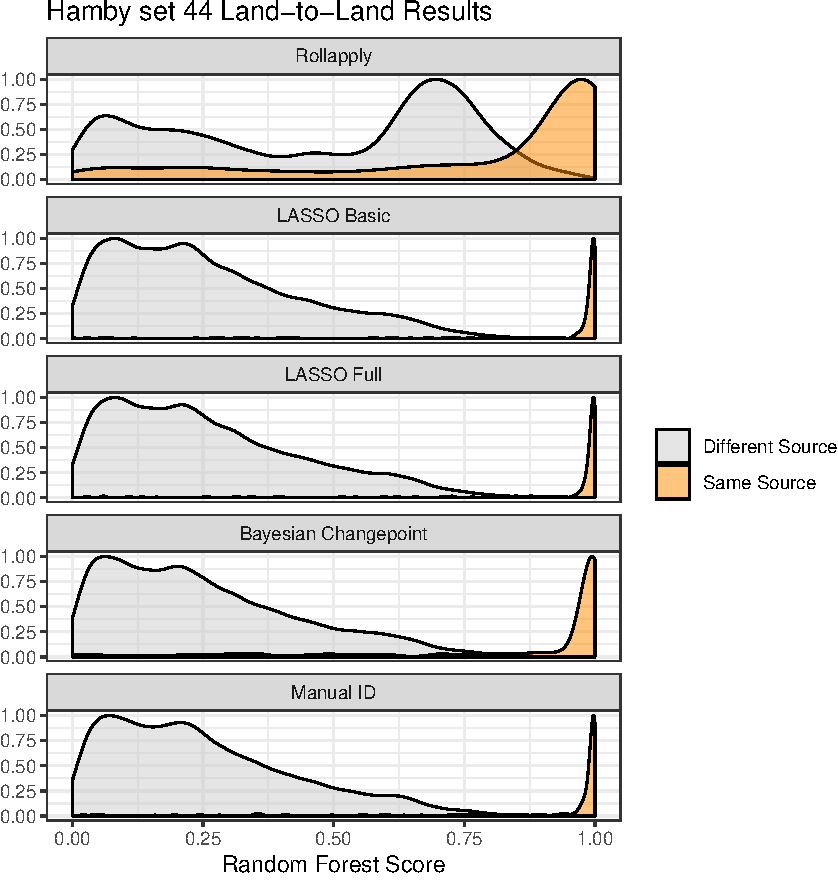
\includegraphics{writeup_files/figure-latex/hamby-groove-results-1.pdf}
\caption{\label{hamby-groove-results}Random forest score distributions
for same source and different source land-to-land comparisons for Hamby
set 44. Distributions should ideally separate between same source and
different source pairs. LASSO Basic, LASSO Full and Bayesian changepoint
all demonstrate significant improvement over Rollapply.}
\end{figure}

\begin{table}[]
\centering
\begin{tabular}{llllllll}
& & \multicolumn{5}{c}{\textbf{Controlled FPR = .01}} & \\
\textbf{Method} & \textbf{AUC} & Cutoff & FN &TP & TN & Accuracy & \textbf{Time to Calculate} \\ \hline
Rollapply & 0.8 &  0.92 & 332 & 420&42126 & 0.98 & 1 min.\\ \hline
LASSO basic & 0.94 &  0.75 &126 & 626&42098 & 0.99 & 6 min. \\ \hline
LASSO full & 0.94 &  0.75 &126 &626 &42106 & 0.99 & 6 min. \\ \hline
Bayesian Changepoint & 0.93 &  0.74 &152 & 600&42098 & 0.99 & \\ \hline
Manual ID & 0.94 & 0.74 & 124& 628&42088 & 0.99 & 45 min. \\ \hline 
\end{tabular}
\caption{Land-to-land comparison results for Hamby set 44.}
\label{hamby-table}
\end{table}

\begin{figure}
\centering
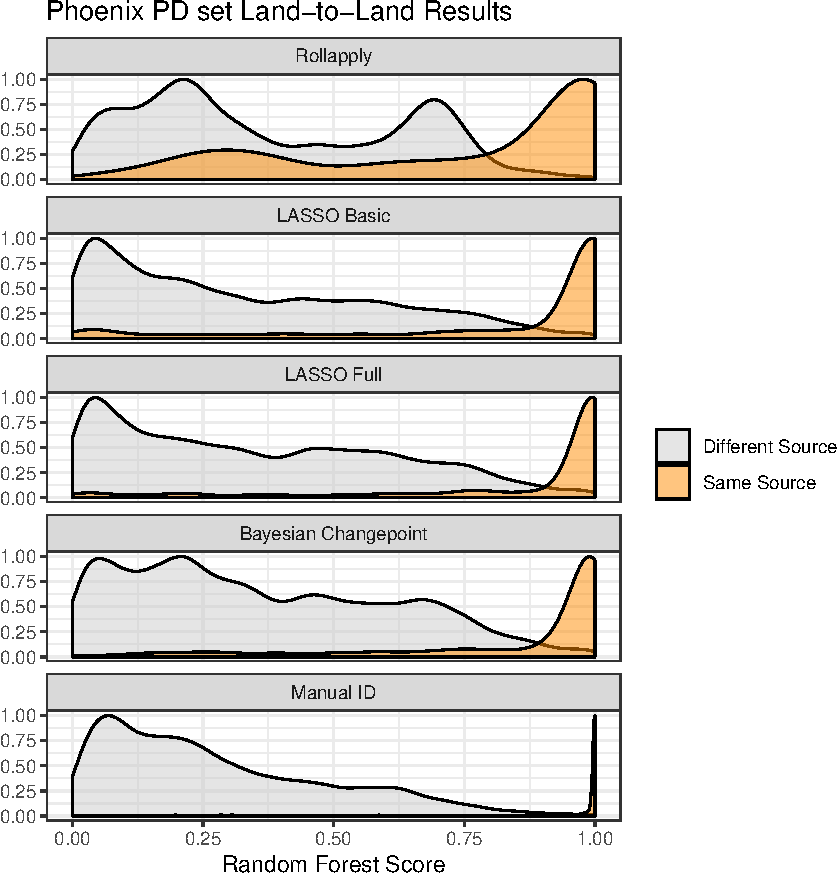
\includegraphics{writeup_files/figure-latex/phoenix-groove-results-1.pdf}
\caption{\label{phoenix-groove-results}Random forest score distributions
for same source and different source land-to-land comparisons for the
Phoenix PD set. LASSO Basic, LASSO Full, and Bayesian changepoint all
demonstrate significant improvement over Rollapply, but are still not as
well separated as the Manual ID distributions.}
\end{figure}

\begin{table}[]
\centering
\begin{tabular}{llllllll}
& & \multicolumn{5}{c}{\textbf{Controlled FPR = .01}} & \\
\textbf{Method} & \textbf{AUC} & Cutoff & FN &TP & TN & Accuracy & \textbf{Time to Calculate} \\ \hline
Rollapply & 0.818 &  0.9 & 364 & 378&38082 & 0.981& 1 min. \\ \hline
LASSO basic & 0.877 &  0.947 &256 & 486&38088 & 0.9839 & 6 min. \\ \hline
LASSO full & 0.893 &  0.953 &238 &504 &38082 & 0.9842  & 6 min. \\ \hline
Bayesian Changepoint & 0.903 &  0.937 &256 & 486&38080 & 0.9837 &  \\ \hline
Manual ID & 0.953 &  0.853 & 96& 646&38084 & 0.9879 & 45 min. \\ \hline 
\end{tabular}
\caption{Land-to-land comparison results for the Phoenix PD set.}
\label{phoenix-table}
\end{table}

\begin{figure}
\centering
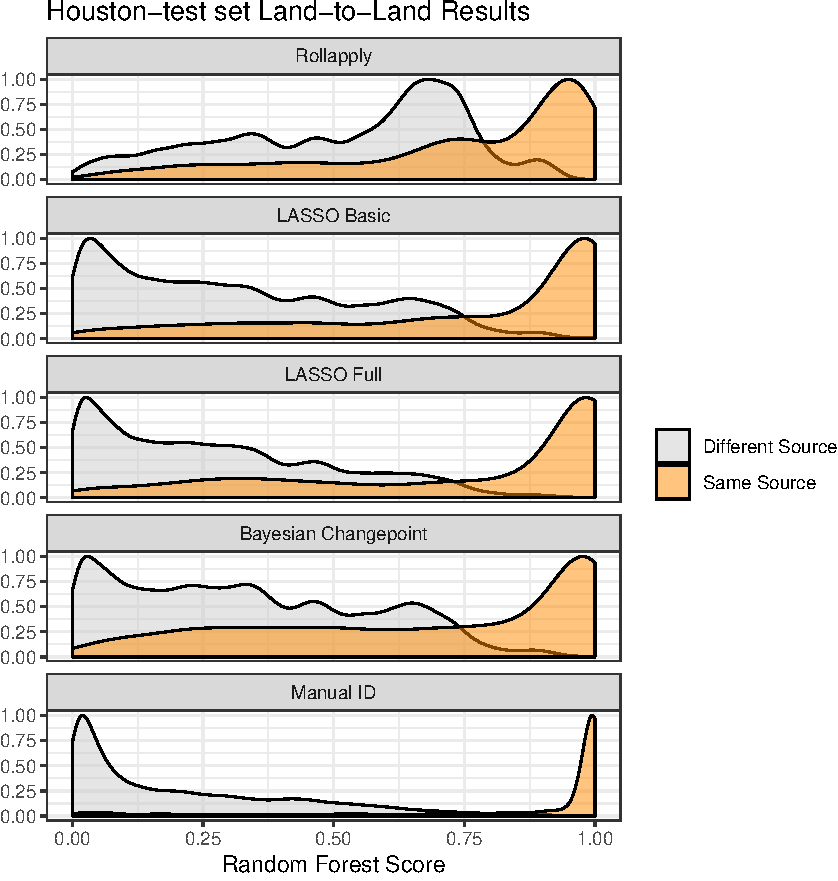
\includegraphics{writeup_files/figure-latex/houston-groove-results-1.pdf}
\caption{\label{houston-groove-results}Random forest score distributions
for same source and different source land-to-land comparisons for the
Houston-test set. LASSO Basic and LASSO Full both demonstrate
improvement over Rollapply, but are still not as well separated as the
Manual ID distributions. Bayesian changepoint demonstrates minor
improvement, but does not improve as much as the LASSO methods.}
\end{figure}

\begin{table}[]
\centering
\begin{tabular}{llllllll}
& & \multicolumn{5}{c}{\textbf{Controlled FPR = .01}} & \\
\textbf{Method} & \textbf{AUC} & Cutoff & FN &TP & TN & Accuracy & \textbf{Time to Calculate} \\ \hline
Rollapply & 0.761 &  0.91 & 1652 & 1016&167118 & 0.981 & 2 min. \\ \hline
LASSO basic & 0.852 &  0.88 &1274 & 1394&167136 & 0.9833 & 12 min. \\ \hline
LASSO full & 0.858 &  0.823 &1144 &1524 &167062 & 0.9836 & 12 min. \\ \hline
Bayesian Changepoint & 0.795 &  0.863 &1552 & 1116&167096 & 0.9814 & \\ \hline
Manual ID & 0.931 &  0.823 & 614& 2054&167098 & 0.9869 & 75 min. \\ \hline 
\end{tabular}
\caption{Land-to-land comparison results for the Houston-test set.}
\label{houston-table}
\end{table}

\section{Conclusions}

All three proposed approaches show significant improvement both visually
and quantitatively over the ``rollapply'' method proposed by
\cite{Hare1}. However, both LASSO methods show greater improvement than
Bayesian changepoint on the Houston-test set. While manual
identification of shoulder locations is still the most accurate method,
and considered the ``gold standard'', the reduction in time to get
predictions when using LASSO methods is advantageous and allows for less
human involvement in the overall automated matching process.

While improvement is apparent on all three test sets using the LASSO and
Bayesian changepoint methods, future work on the LASSO methods should
include re-training LASSO models on a wider variety of LEA types rather
than just the Hamby set 44 to avoid over-fitting to a specific type of
LEA.

\kr{Nate, could you add some conclusions about BCP stuff here? A sentence or two?}

\section{References}

\section{Appendix}

\subsection{MCMC Details}

As a practical note, it turns out that the posterior distribution is
almost always multimodal, and it can happen that the sampler gets stuck
in a suboptimal mode for a large number of iterations. It is also the
case that the suboptimal modes need not even be close to the groove
locations. It has, however, been our experience that the optimal mode
corresponds well to the actual groove locations, which are often
somewhat close to the edges of the data. With this in mind, starting
values and the RWMH proposal variances play a very important role in the
success of the sampling algorithm. Fortunately, it seems to be the case
that by setting the initial changepoint values close to the edges of the
data and making the proposal variance small (around 100 seems to work
well) allows the sampler to wander inwards, and even with a modest
number of iterations (say 5000), typically pass through the largest mode
corresponding to the groove locations. This is not always the case, and
it is possible that increasing the number of iterations produces better
results.

In our implementation of this algorithm, the sampling functions were
originally written with the intention of tuning the proposal variances
to potentially accelerate convergence, and thus several warmup
iterations are required for this purpose. This turns out to be a bad
idea in this context for two reasons. The first reason is that the
warmup iterations allow the sampler to wander past the global modes and
get stuck in suboptimal modes far from the groove locations, from which
the sampler may or may not find its way back to the optimal modes in
just a few thousand iterations. Secondly, if the sampler does wander
past the optimal modes, which are usually on the edges of the data, the
tuned proposal variance can be quite large. The large proposal variance
might not be a huge problem if it weren't for the fact that the width of
the modes are almost always quite small. This means that it can take a
very, very long time for the sampler to move from a suboptimal mode to
the global mode. In order to mitigate this problem, we are currently
setting the number of warmup iterations to be relatively small
(somewhere in 100 to 500 seems to work well). In future, our
implementation of the algorithm will not require any warmup iterations.

Initially, the Metropolis proposal variance for each \(\theta_i\) is
diagonal with diagonal elements all equal to \(1/2\). The proposal
variance for \((c_l, c_r)\) is initially set to be diagonal with
elements equal to \(10^2\). Note that because of the currently necessary
warmup iterations, the variances after warmup for each \(\theta_i\)
becomes
\(\frac{2.4^2}{d}\hat{Var}(\theta_i^{(1:w)}) + \text{diag}(0.1)\), where
\(d\) is the dimension of \(\theta_i\) (which is not constant between
GEAs and LEA), and \(\hat{Var}(\theta_i^{(1:w)})\) is the estimated
variance covariance matrix from the \(w\) warmup iterations. Note that
the addition of a diagonal matrix with entries \(0.1\) is to avoid the
case when most or all warmup iterations have the same value. Similarly,
the proposal variance for \((c_l, c_r)\) after warmup becomes
\(\frac{2.4^2}{2}\hat{Var}((c_l,c_r)^{(1:w)}) + \text{diag}(1)\).

\subsection{Data Preprocessing for MCMC}

Before running the MCMC to do the changepoint detection, we first
perform two data preprocessing steps. The first step is to scale the
residuals from the robust loess procedure by the standard deviation
calculated from the entire set of residuals. The reason for this is
simply to make priors for standard deviation and slope parameters easier
to specify. For example, ensuring that the residuals are scaled to have
standard deviation one means that the standard deviation parameters in
our model should also be close to one. This scaling also ensures that
slopes values are not very large.

The second preprocessing step is a bit more involved. In order to enable
the algorithm to run reasonably fast, we need to take advantage of the
sparse precision matrix structure that is induced by the exponential
covariance function. Indeed, this was the reason for choosing this
covariance function in the first place. Unfortunately, it is challenging
to do this unless the observations are evenly spaced in the domain. In
our case, this would be true if there were no missing values. In order
to remedy this problem, we impute the missing data, but only in the case
that there exist nonmissing observations outside of the missing values.
In the case that the missing values exist on the edges of the data, we
simply do not consider those domain values in the model.

We perform the imputation by treating the observations as coming from an
unknown function, and infer the missing values from the known function
values. In order to do this, we model the data with a Gaussian process
and the squared exponential covariance function. That is, we suppose
that

\[
Y(x) \sim \mathcal{GP}(0, K(x,x';\sigma^2, \ell)),
\]

\noindent where now
\(K(x,x';\sigma^2, \ell) = \sigma^2 e^{-(x - x')^2/(2\ell^2)}\) is the
squared exponential covariance function. We emphasize for clarity that
this is a different covariance function than we use in the changepoint
model. The main reason for this is that in imputing values, it seems
desireable to allow dependencies beyond immediately neighboring points
to influence predictions as the function that we are trying to predict
generally has a smooth global structure. For all of our experiments, we
set \(\sigma = 0.8\) and \(\ell = 15\). These values were chosen from
doing maximum likelihood estimation for a representative bullet.

When we impute the missing values, we compute the conditional mean of
the missing values. To be clear, denote the distribution of the observed
and missing data as

\[ 
(Y,Y^*)^\top \sim N\left( \begin{bmatrix} 0 \\ 0 \end{bmatrix}, \begin{bmatrix} \Sigma_{yy} & \Sigma_{yy^*} \\ \Sigma_{y^*y} & \Sigma_{y^*y^*}\end{bmatrix} \right).
\]

\noindent Here, \(Y\) is observed data and \(Y^*\) is the missing data,
and the covariance matrix above is constructed from the squared
exponential covariance function. We then use normal distribution theory
to calculate the imputed values

\[ E(Y^*|Y = y) = \Sigma_{y^*y} \Sigma_{yy}^{-1}y \].

\bibliographystyle{jfs-authoryear}
\bibliography{bibliography}

\end{document}